\begin{figure}[H]
\centering
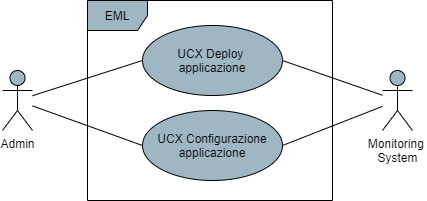
\includegraphics[scale=0.6]{res/UseCase/Immagini/Admin}
\caption{Diagramma UML per i casi d'uso riguardanti l'attore admin}
\end{figure}

\subsubsection{UC13 - Deploy applicazione}
\begin{itemize}
\item \textbf{Attori primari}: admin;
\item \textbf{Descrizione}: l'admin può effettuare il deploy dell'applicazione;
\item \textbf{Scenario Principale}: l'admin, attraverso una piattaforma di monitoraggio dell'applicazione, può eseguire i deploy di essa;
\item \textbf{Precondizione}: l'admin si trova nella piattaforma di gestione dell'applicazione;
\item \textbf{Postcondizione}: l'admin esegue il deploy dell'applicazione.
\end{itemize}

\subsubsection{UC14 - Configurazione applicazione}
\begin{itemize}
\item \textbf{Attori primari}: admin;
\item \textbf{Descrizione}: l'admin può gestire e configurare l'applicazione, compresa di integrazioni di terze parti che essa utilizza;
\item \textbf{Scenario Principale}: l'admin, attraverso una piattaforma di monitoraggio, può gestire e configurare l'applicazione e le sue integrazioni di terze parti utilizzate.
\item \textbf{Precondizione}: l'admin si trova nella piattaforma di gestione dell'applicazione;
\item \textbf{Postcondizione}: l'admin ha gestito e configurato l'applicazione a suo piacimento.
\end{itemize}

